\chapter{Конструкторский раздел}

В данном разделе описаны структура разрабатываемого ПО, используемые структуры данных, а также приведены схемы алгоритмов используемых при отрисовке изображения.

\section{Структура ПО}

\subsection{Иерархия классов}

Ниже приведена иерархия классов для архитектурного домена. (лучше вынести в приложение)

\begin{figure}
	\centering
	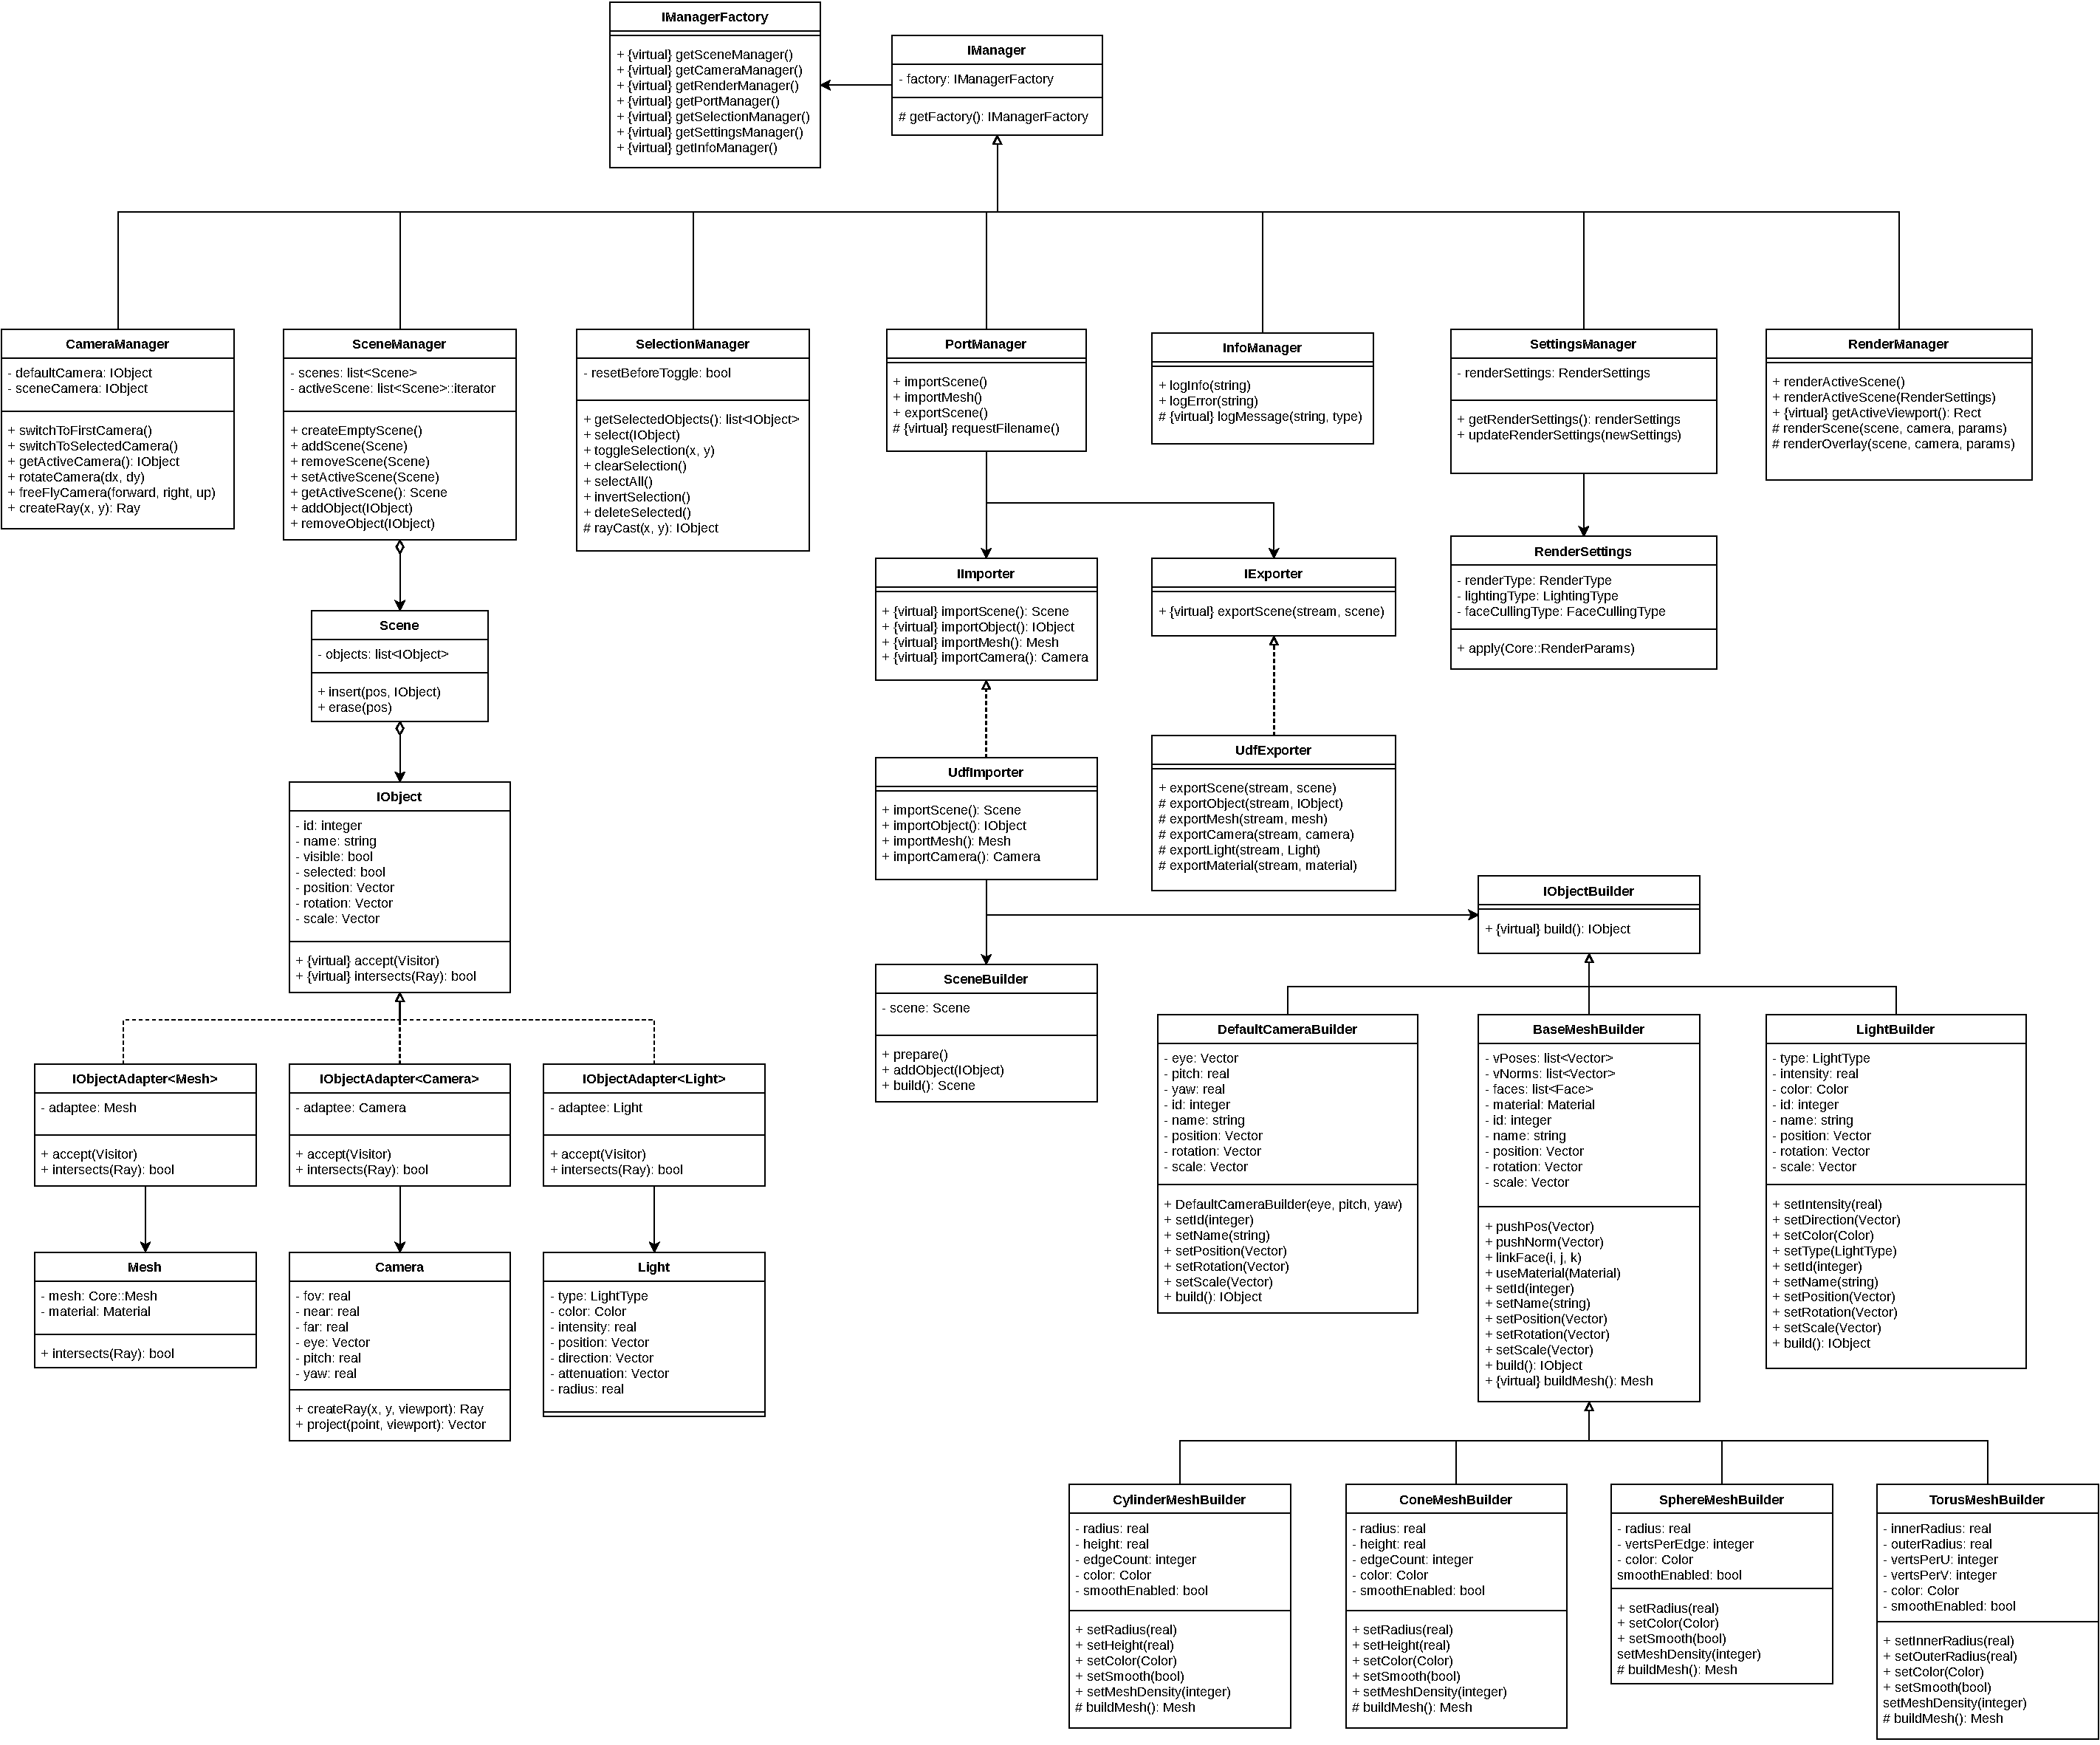
\includegraphics[angle=90,origin=c,width=\linewidth,height=0.85\textheight,keepaspectratio]{diagrams/uml.pdf}
\end{figure}

\subsection{Процесс синтеза изображения}

Ниже представлена IDEF0 диаграмма процесса синтеза изображения сцены.

\begin{figure}
    \centering
    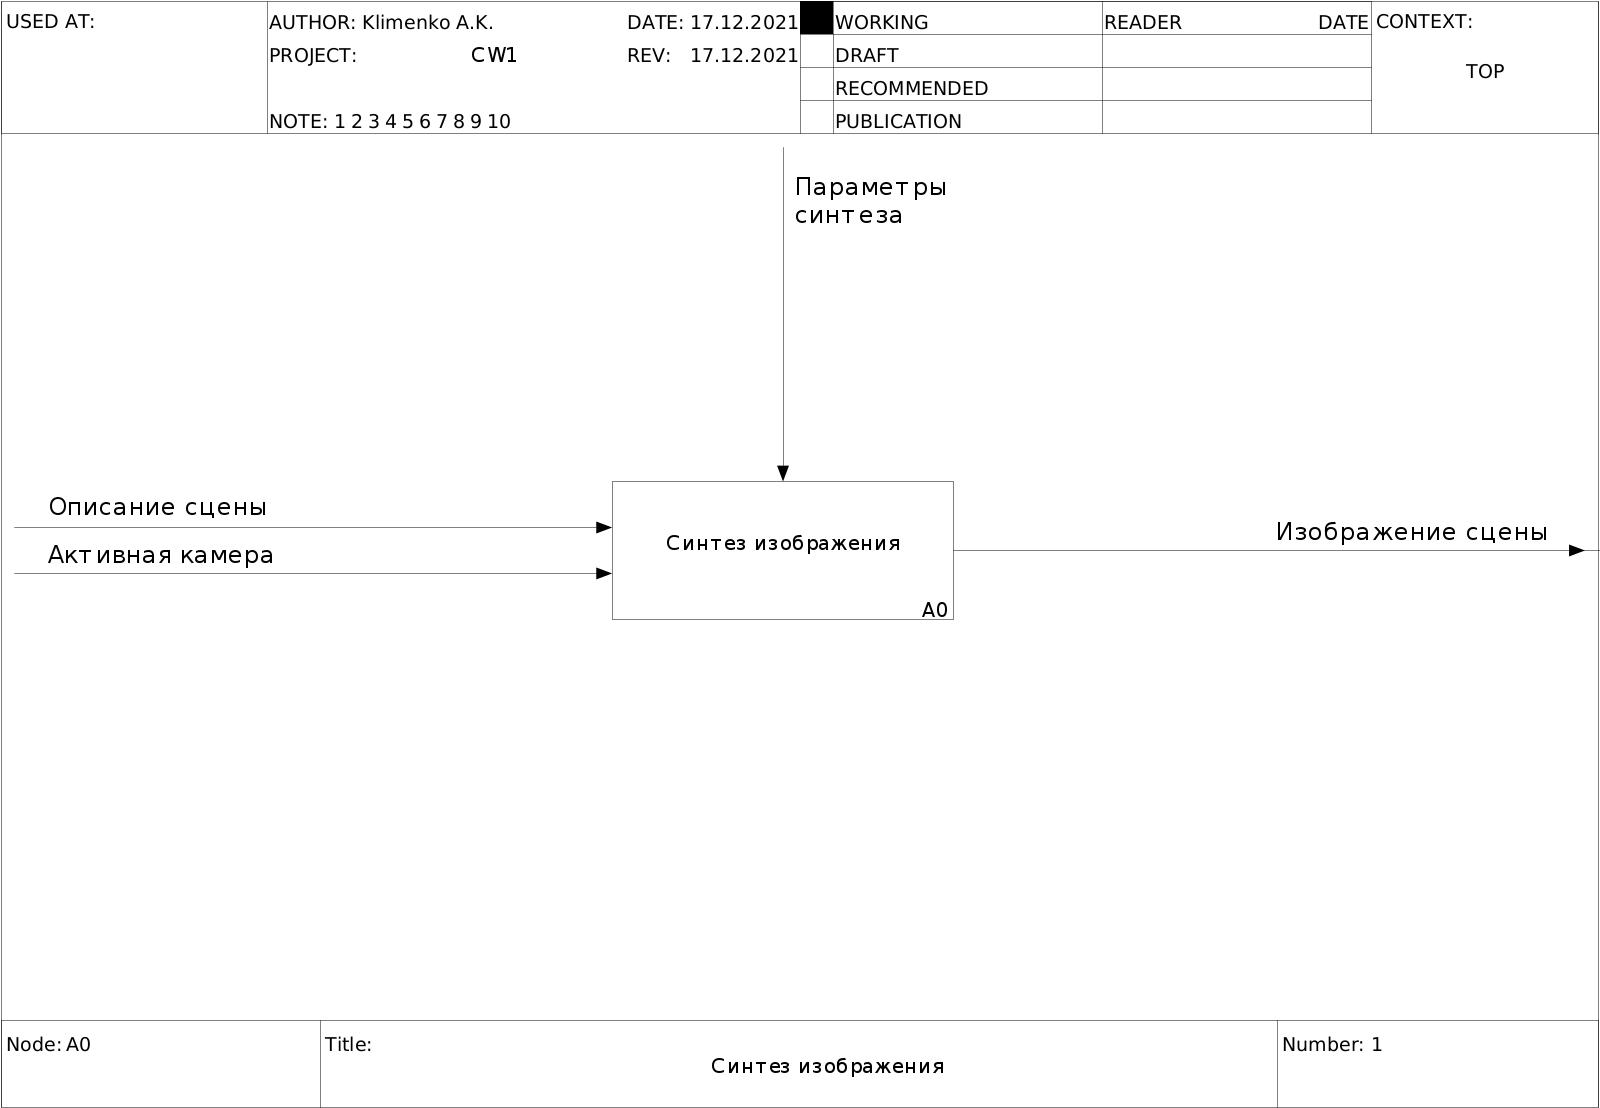
\includegraphics[width=\linewidth,height=0.85\textheight,keepaspectratio]{idef0/01_A0.jpg}
\end{figure}

\begin{figure}
    \centering
    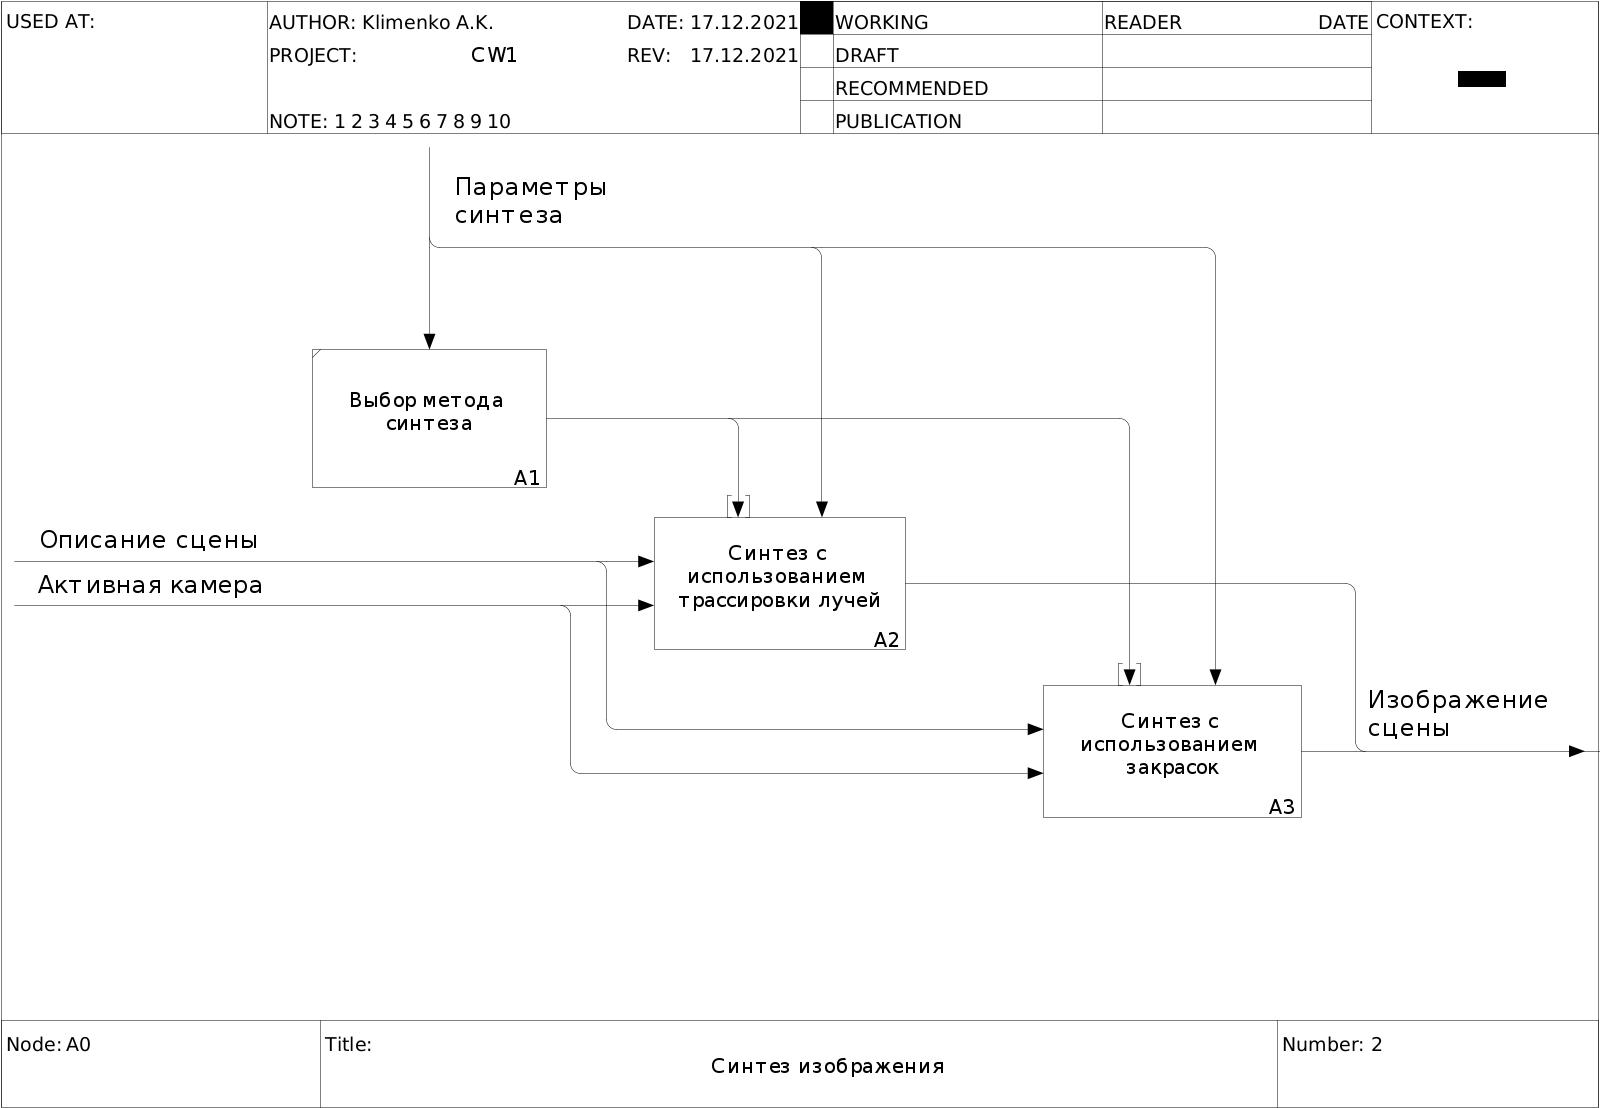
\includegraphics[width=\linewidth,height=0.85\textheight,keepaspectratio]{idef0/02_A0.jpg}
\end{figure}

\begin{figure}
    \centering
    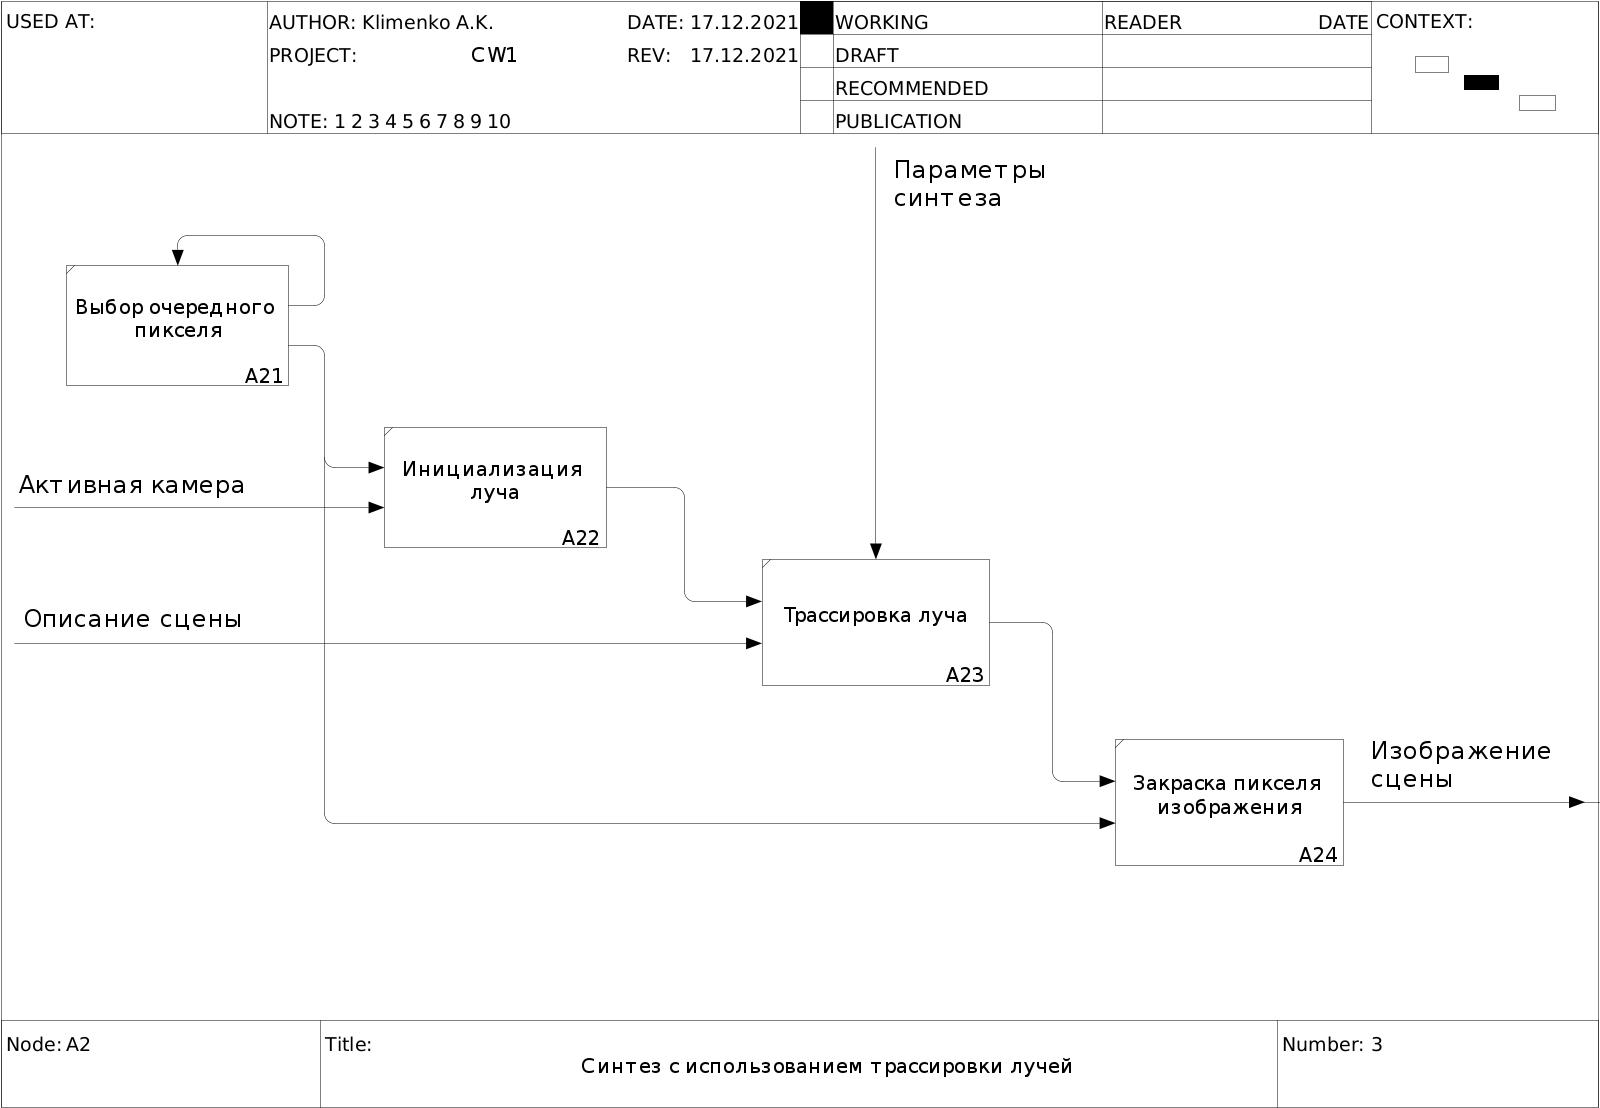
\includegraphics[width=\linewidth,height=0.85\textheight,keepaspectratio]{idef0/03_A2.jpg}
\end{figure}

\begin{figure}
    \centering
    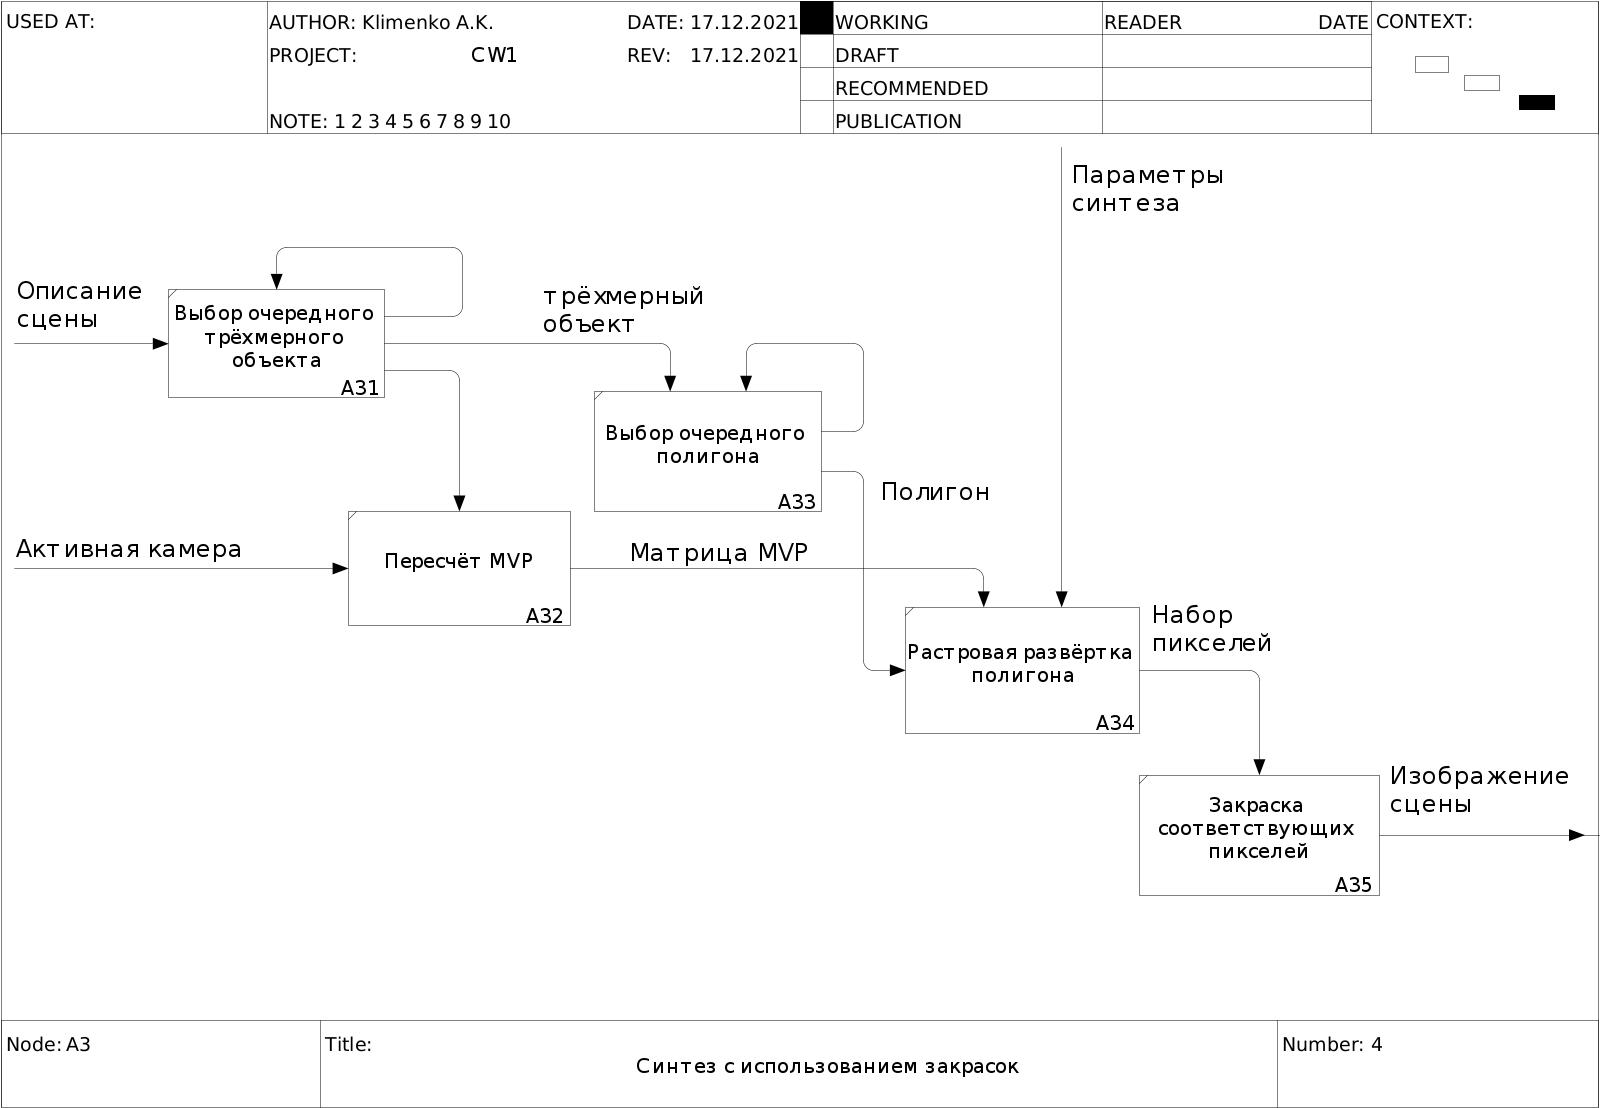
\includegraphics[width=\linewidth,height=0.85\textheight,keepaspectratio]{idef0/04_A3.jpg}
\end{figure}

\clearpage

\section{Схемы алгоритмов}

В данной секции представлены 2 алгоритма синтеза изображения. Первый использует закраски полигонов, а второй -- метод трассировки лучей.

\subsection{Быстрая отрисовка}

\begin{figure}
	\centering
	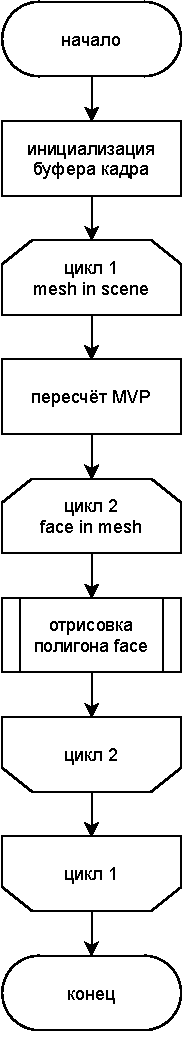
\includegraphics[width=\linewidth,height=\textheight,keepaspectratio]{diagrams/fast.pdf}
\end{figure}

\begin{figure}
	\centering
	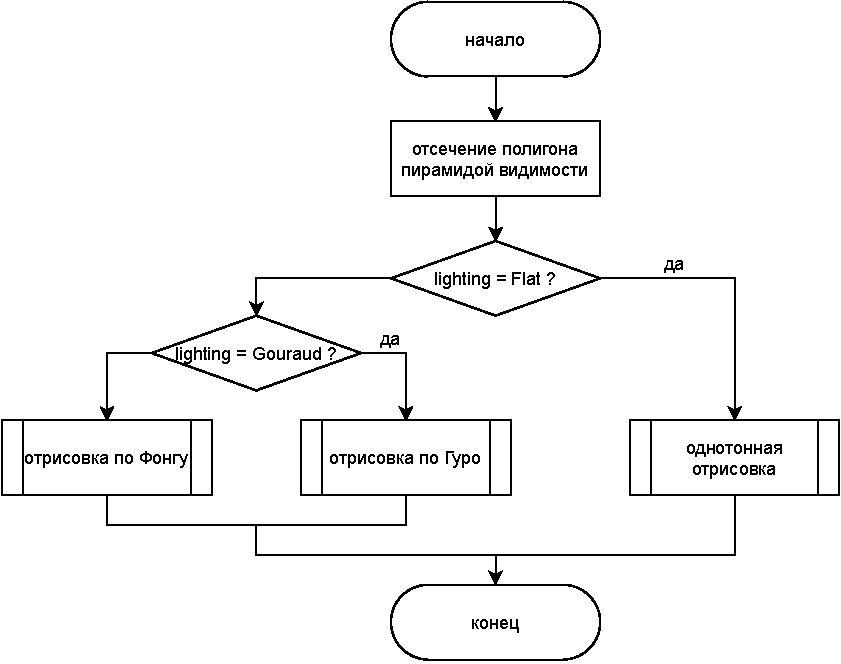
\includegraphics[width=\linewidth,height=\textheight,keepaspectratio]{diagrams/draw-face.pdf}
\end{figure}

\subsection{Реалистичная отрисовка}

\begin{figure}
	\centering
	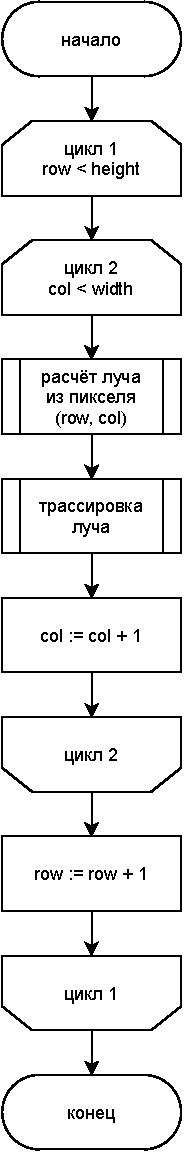
\includegraphics[width=\linewidth,height=\textheight,keepaspectratio]{diagrams/fancy.pdf}
\end{figure}

\clearpage

\section{Структуры данных}

В данной подсекции описываются основные структуры данных, необходмые для решения задачи синтеза изображения.

\subsection{Сцена}

В рассматриваемой задаче синтеза изображения сцена является элементом самого верхнего уровня, в полной мере содержащим информацию об объектах, находящихся на сцене, а также информацию об используемом освещении.

Данная структура данных будет использоваться прежде всего для отображения объектов, поэтому основным требованием, предъявляемым к ней, будет эфективная выборка объектов сцены. Из этого можно заключить, что наиболее выгодным с точки зрения производительности будет выбор массива в качестве контейнера для объектов сцены и источников освещения.

\subsection{Трёхмерное тело}

Рассматривая задачу синтеза изображения, любое трёхмерный объект можно разложить на две составляющие -- форму тела (его геометрию), и оптические свойства поверхности материала, из которого изготовлен объект.

Выбор структуры трёхмерного тела должен выполняться в соответствии с выбранными алгоритмами решения поставленной задачи. В следствии чего было принято решение об использовании массива треугольников в качестве описания геометрии объекта.

Оптические свойства поверхности объекта будут описаны в отдельной структуре -- материал. Она будет включать в себя такие параметры, как: цвет фонового освещения, цвет направленного освещения, цвет бликов. Также данная структура будет содержать следующие параметры для синтеза реалистичного изображения: коэффициенты прозрачности, отражния и преломления, а также показатель преломления среды.

\subsection{Источник освещения}

В постановке задачи синтеза изображения выделены следующие типы источников освещения: фоновый, направленный и точечный. Далее каждый тип будет рассмотрен в отдельности.

\textbf{Фоновое освещение.} Фоновая освещённость объектов в сцене не зависит от положения источника света в пространстве, а зависит только от цвета освещения и его интенсивности.

\textbf{Направленное освещение.} Для данного типа освещения необходимо хранить его цвет, интенсивность и направление.

\textbf{Точечное освещение.} ...

%\section{Тестирование ПО}
